\section{Global Trigger Logic}
\label{sec:gtl:global_trigger_logic}

This description is for version \versiongtl of Global Trigger Logic.\\

The Global Trigger Logic (\ugtl) firmware contains conditions and algorithms for trigger decision (see Figure \ref{fig:gtl:mGTL_firmware}).

Definitions are based on document~\cite{interface}.

\begin{figure}[htb]
\centering
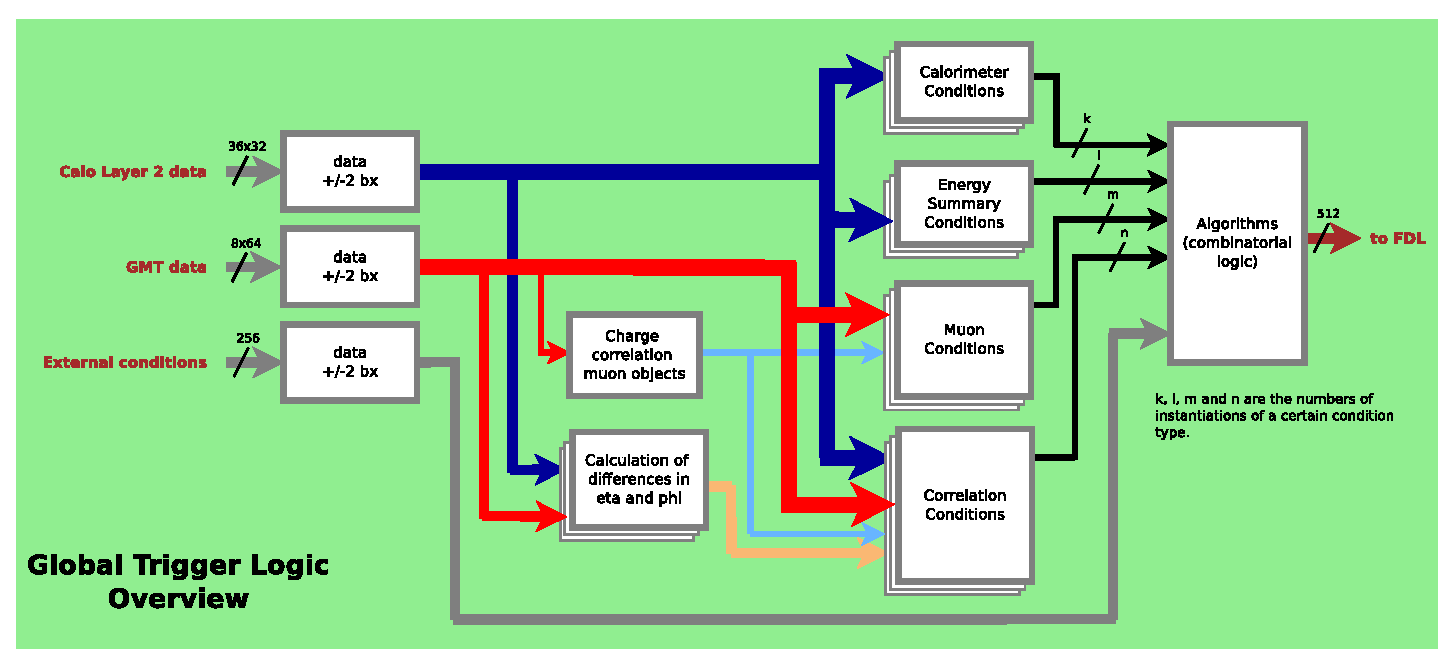
\includegraphics[width=15cm]{figures/mGTL_firmware}
\caption{\ugtl firmware}
\label{fig:gtl:mGTL_firmware}
\end{figure}

\subsection{\ugtl Interface}
\label{sec:gtl:ugtl_interface}

\textbf{Inputs:}
\begin{itemize}
\item Calo-Layer2 data
\begin{itemize}
\item Electron/$\gamma$ objects (EG0..EG11)
\item Jet objects (JET0..JET11)
\item Tau objects (TAU0..TAU11)
\item Energy summary information:
\begin{itemize}
\item Total Et (\ett)
\item Total Et from ECAL only (ETTEM)
\item Total calibrated Et in jets (\htt)
\item Missing Et (\etm)
\item Missing Et including HF (ET$_{miss}^{HF}$)
\item Missing Ht objects (\htm)
\item Missing Ht including HF (HT$_{miss}^{HF}$)
\item "Asymmetry" information (ASYMET, ASYMHT, ASYMETHF, ASYMHTHF)
\end{itemize}
\item Minimum bias HF bits (MBT0HFP, MBT0HFM, MBT1HFP and MBT1HFM; part of energy summary information data structure)
\item Towercount bits (TOWERCOUNT, number of firing HCAL towers; part of energy summary information data structure)
\item "Centrality" bits (CENT0..CENT7; part of energy summary information data structure)
\end{itemize}
\item \gmt data
\begin{itemize}
\item Muon objects (MU0..MU7)
\item Muon shower bits (bit 61 on MU0, MU2, MU4, MU6)
\end{itemize}
\item External conditions
\end{itemize}
\textbf{Outputs:}
\begin{itemize}
\item Algorithms
\end{itemize}

\subsection{Definition of optical interfaces}
\label{sec:gtl:optical_interfaces}

\textbf{Remark:}\\
All definitions for scales in the following chapters are from a CMS Detector Note: "Scales for inputs to $\mu$GT" (see~\cite{interface}).

\subsubsection{Calo-Layer2 optical interface}
\label{sec:gtl:gct_optical_interfaces}

The data structure of an \egamma object (bits 27..31 are not defined yet, reserved for quality, ...):
\begin{center}
\begin{bytefield}[boxformatting={\centering\itshape}, bitwidth=1.2em, endianness=big]{32}
        \bitheader{0,8,9,16,17,24,25,26,27,31} \\
        \bitbox {5}     {\texttt{qual/spare}} &
        \bitbox {2}     {\texttt{iso}} &
        \bitbox {8}     {\texttt{$\varphi$}}  &
        \bitbox {8}     {\texttt{$\eta$}}  &
        \bitbox {9}     {\texttt{\et}} \\
\end{bytefield}
\end{center}

The data structure of a jet object:\\
\tiny{Remark: "D" means DISP bit (displaced jet) - "qu" means quality flags - "sp" means spare bits.}\normalsize
\begin{center}
\begin{bytefield}[boxformatting={\centering\itshape}, bitwidth=1.2em, endianness=big]{32}
        \bitheader{0,10,11,18,19,26,27,27,28,29,30,31} \\
        \bitbox {2}     {\texttt{sp}} &
        \bitbox {2}     {\texttt{qu}} &
        \bitbox {1}     {\texttt{D}} &
        \bitbox {8}     {\texttt{$\varphi$}}  &
        \bitbox {8}     {\texttt{$\eta$}}  &
        \bitbox {11}    {\texttt{\et}} \\
\end{bytefield}
\end{center}

The data structure of a tau object (bits 27..31 are not defined yet, reserved for quality, ...):
\begin{center}
\begin{bytefield}[boxformatting={\centering\itshape}, bitwidth=1.2em, endianness=big]{32}
        \bitheader{0,8,9,16,17,24,25,26,27,31} \\
        \bitbox {5}     {\texttt{qual/spare}} &
        \bitbox {2}     {\texttt{iso}} &
        \bitbox {8}     {\texttt{$\varphi$}}  &
        \bitbox {8}     {\texttt{$\eta$}}  &
        \bitbox {9}     {\texttt{\et}} \\
\end{bytefield}
\end{center}

The data structure of "Total Et" (\ett) quantity [including "Total Et from ECAL only" (ETTEM) and "minimum bias HF+ threshold 0" bits]:
\begin{center}
\begin{bytefield}[boxformatting={\centering\itshape}, bitwidth=1.2em, endianness=big]{32}
        \bitheader{0,11,12,23,24,27,28,31} \\
        \bitbox {4}    {\texttt{MBT0HFP}} &
        \bitbox {4}    {\texttt{spare}} &
        \bitbox {12}    {\texttt{\et [ETTEM]}} &
        \bitbox {12}    {\texttt{\et [\ett]}} \\
\end{bytefield}
\end{center}

The data structure of "Total calibrated Et in jets" (\htt) quantity [including "towercount" and "minimum bias HF- threshold 0" bits]:
\begin{center}
\begin{bytefield}[boxformatting={\centering\itshape}, bitwidth=1.2em, endianness=big]{32}
        \bitheader{0,11,12,24,25,27,28,31} \\
        \bitbox {4}    {\texttt{MBT0HFM}} &
        \bitbox {3}    {\texttt{spare}} &
        \bitbox {13}    {\texttt{TOWERCOUNT}} &
        \bitbox {12}    {\texttt{\et}} \\
\end{bytefield}
\end{center}

The data structure of "Missing Et" (\etm) quantity [including "Asymmetry" ASYMET and "minimum bias HF+ threshold 1" bits]:
\begin{center}
\begin{bytefield}[boxformatting={\centering\itshape}, bitwidth=1.2em, endianness=big]{32}
        \bitheader{0,11,12,19,20,27,28,31} \\
        \bitbox {4}    {\texttt{MBT1HFP}} &
        \bitbox {8}    {\texttt{ASYMET}} &
        \bitbox {8}     {\texttt{$\varphi$}} &
        \bitbox {12}    {\texttt{\et}} \\
\end{bytefield}
\end{center}

The data structure of "Missing Ht" (\htm) quantity [including "Asymmetry" ASYMHT and "minimum bias HF- threshold 1" bits]:
\begin{center}
\begin{bytefield}[boxformatting={\centering\itshape}, bitwidth=1.2em, endianness=big]{32}
        \bitheader{0,11,12,19,20,27,28,31} \\
        \bitbox {4}    {\texttt{MBT1HFM}} &
        \bitbox {8}    {\texttt{ASYMHT}} &
        \bitbox {8}     {\texttt{$\varphi$}} &
        \bitbox {12}    {\texttt{\et}} \\
\end{bytefield}
\end{center}

The data structure of "Missing Et including HF" (ET$_{miss}^{HF}$) quantity [including "Asymmetry" ASYMETHF and "Centrality" bits (3:0)]:
\begin{center}
\begin{bytefield}[boxformatting={\centering\itshape}, bitwidth=1.2em, endianness=big]{32}
        \bitheader{0,11,12,19,20,27,28,31} \\
        \bitbox {4}    {\small  \texttt{[CENT3:0]}} &
        \bitbox {8}    {\texttt{ASYMETHF}} &
        \bitbox {8}     {\texttt{$\varphi$}} &
        \bitbox {12}    {\texttt{\et}} \\
\end{bytefield}
\end{center}

The data structure of "Missing Ht including HF" (HT$_{miss}^{HF}$) quantity [including "Asymmetry" ASYMHTHF and "Centrality" bits (7:4)]:
\begin{center}
\begin{bytefield}[boxformatting={\centering\itshape}, bitwidth=1.2em, endianness=big]{32}
        \bitheader{0,11,12,19,20,27,28,31} \\
        \bitbox {4}    {\small  \texttt{CENT[7:4]}} &
        \bitbox {8}    {\texttt{ASYMHTHF}} &
        \bitbox {8}     {\texttt{$\varphi$}} &
        \bitbox {12}    {\texttt{\et}} \\
\end{bytefield}
\end{center}

\subsubsection{\gmt optical interface}
\label{sec:gtl:gmt_optical_interfaces}

The data structure of a muon object (64 bits):\\
\tiny{Remark: "extrapol." means extrapolated - "qual" means quality bits - "iso" means isolation bits - "ch" means charge bits (bit 34 = charge sign, bit 35 = charge valid) - "m" means muon shower bit (on MU0 [MUS0], MU2 [MUS1], MU3 [MUS2], MU4 [MUSOOT0] and MU6 [MUSOOT1]; spare on MU1, MU5 and MU7) - "imp" = impact parameter.}\normalsize
\begin{center}
\begin{bytefield}[boxformatting={\centering\itshape}, endianness=big, bitwidth=1.2em]{32}
        \bitheader[lsb=32]{32,33,34,35,36,42,43,52,53,60,61,61,62,63} \\
        \bitbox {2}     {\small  \texttt{imp}}       &
        \bitbox {1}     {\small  \texttt{m}}       &
        \bitbox {8}     {\texttt{unconst.\pt}}       &
        \bitbox {10}    {\texttt{$\varphi$} (out)}
        \bitbox {7}     {\texttt{index bits}}
        \bitbox {2}     {\small  \texttt{ch}}       &
        \bitbox {2}     {\small \texttt{iso}} \\
        [3ex]
        \bitheader{0,9,10,18,19,22,23,31} \\
        \bitbox {9}     {\texttt{$\eta$} (extrapol.)}       &
        \bitbox {4}     {\texttt{qual}}       &
        \bitbox {9}     {\texttt{\pt}}    &
        \bitbox {10}    {\texttt{$\varphi$} (extrapol.)} \\
\end{bytefield}
\end{center}

\clearpage

\subsection{Implementation in firmware}
\label{sec:gtl:implementation_firmware_gtl}

The firmware of \ugtl consists of two main parts:
\begin{itemize}
\item A top-of-hierarchy module \href{\gitbranch/firmware/hdl/payload/gtl\_module\_tpl.vhd}{\texttt{\textquotesingle gtl\_module.vhd\textquotesingle }}, which contains the pipeline for $\pm$2bx data, the instantiations of calculators for differences in $\eta$ and $\varphi$, the instantiations of conditions, the instantiations of charge correlation logic of muons and the Algorithms logic for 512 Algorithms, as well as a package file (\href{\gitbranch/firmware/hdl/packages/gtl\_pkg.vhd}{\texttt{\textquotesingle gtl\_pkg.vhd\textquotesingle }}) for declarations.
Currently 6 AMC (MP7) boards are used to contain Algorithms.\\
A software tool called Trigger Menu Editor (TME)~\cite{TME_repo} is available to create a L1Menu with up to 512 Algorithms, which are partitioned by VHDL Producer~\cite{VHDL_Producer} to the 6 MP7 boards.\\
The VHDL Producer creates VHDL snippets files (\texttt{algo\_index.vhd}, \texttt{gtl\_module\_instances.vhd}, \texttt{gtl\_module\_signals.vhd}, \texttt{ugt\_constants.vhd}) for a certain Trigger Menu.\\
These snippets are inserted into templates for \texttt{gtl\_module.vhd} (\href{\gitbranch/firmware/hdl/payload/gtl\_module\_tpl.vhd}{\texttt{\textquotesingle gtl\_module\_tpl.vhd\textquotesingle }}), \texttt{algo\_mapping\_rop.vhd} (\href{\gitbranch/firmware/hdl/payload/fdl/algo_mapping_rop_tpl.vhd}{\texttt{\textquotesingle algo\_mapping\_rop\_tpl.vhd\textquotesingle }}) and \texttt{fdl\_pkg.vhd} (\href{\gitbranch/firmware/hdl/packages/fdl_pkg_tpl.vhd}{\texttt{\textquotesingle fdl\_pkg\_tpl.vhd\textquotesingle }}) during simulation and synthesis (see Figure \ref{fig:gtl:tme_gtl}).
\item A set of VHDL files exists for all the modules instantiated in top-of-hierarchy and the modules in the hierarchy. These files, called the "fixed part", are not influenced by VHDL Producer.
\end{itemize}

\begin{figure}[htb]
\centering
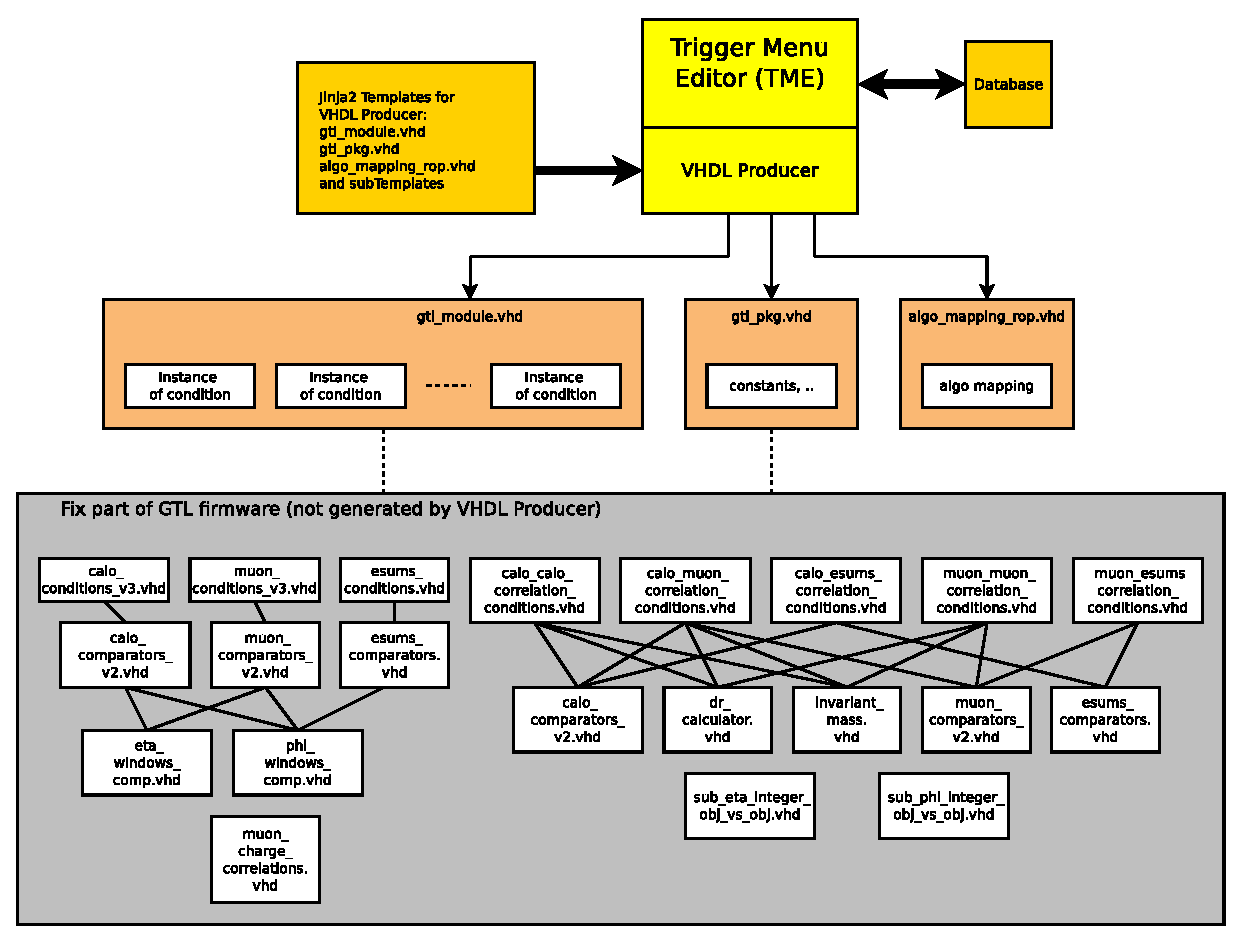
\includegraphics[width=15cm]{figures/tme_gtl}
\caption{VHDL file generation by VHDL Producer}
\label{fig:gtl:tme_gtl}
\end{figure}

The latency of \ugtl is fixed to 5 bunch-crossings: two bunch-crossings for the pipeline of $\pm$2bx data, two bunch-crossings for conditions (fixed, for the conditions requested in the future, too), one bunch-crossing for the logic of Algorithms (see Figure \ref{fig:gtl:gtl_pipeline}).\\

\subsubsection{Top-of-hierarchy module of \ugtl}
\label{sec:gtl:top_module}

The top-of-hierarchy module of \ugtl (\href{\gitbranch/firmware/hdl/payload/gtl\_module\_tpl.vhd}{\texttt{\textquotesingle gtl\_module\_tpl.vhd\textquotesingle }}) contains
\begin {itemize}
\item pipeline for $\pm$2bx data
\item instantiations of charge correlation logic of muons (generated by VHDL Producer)
\item instantiations of calculators for differences in $\eta$ and $\varphi$ (generated by VHDL Producer)
\item instantiations of calculators for $\Delta\eta$ and $\Delta\varphi$ cuts  (generated by VHDL Producer)
\item instantiations of calculators for mass, $\Delta$R and two-body pt cuts  (generated by VHDL Producer)
\item instantiations of conditions (generated by VHDL Producer)
\item boolean logic for Algorithms (generated by VHDL Producer)
\end {itemize}

Listing~\ref{lst:gtl:gtl_module_vhd} contains the entity declaration of the top-of-hierarchy module of \ugtl.

All the declarations for arrays (\textquotesingle type\textquotesingle ), parameters (\textquotesingle constant\textquotesingle ) and look-up-tables (\textquotesingle constant\textquotesingle ) used in modules are available in \href{\gitbranch/firmware/hdl/packages/gtl_pkg.vhd}{\texttt{\textquotesingle gtl\_pkg.vhd\textquotesingle }} package-file.

\clearpage

\lstinputlisting[label=lst:gtl:gtl_module_vhd,language=VHDL,caption=Entity declaration of \texttt{gtl\_module\_tpl.vhd}]{interfaces/gtl_module_tpl.vhd}

\medskip
\begin{table}
\footnotesize
\caption{Explanation of Listing~\ref{lst:gtl:gtl_module_vhd}}
\vspace{5mm}
\centering
\begin{tabular}{l p{.7\columnwidth}}
\toprule
{Item} & {Explanation}\\
\midrule
\verb|lhc_clk| & clock input (LHC clock).\\
\verb|gtl_data| & input data ($\pm$2bx data).\\
\verb|algo_o| & algorithms output.\\
\bottomrule
\end{tabular}
\label{tab:gtl:explanation_fdl_module_vhd}
\end{table}

\clearpage

\subsection{\ugtl structure}
\label{sec:gtl:mgtl_structure}

\subsubsection{Data $\pm$2bx}
\label{sec:gtl:data_p_m_2bx}

The \ugtl input data flow through a register pipeline of four stages. With those data it is possible to have conditions with objects from
different bunch-crossings (within $\pm$2 bunch-crossings), \egamma for Correlation conditions.\\
See Figure \ref{fig:gtl:gtl_pipeline} for a scheme of \ugtl pipeline structure. The data "data\_p\_1bx" and "data\_p\_2bx" occur 1 respectively 2 bunch-crossings
after data for a certain bunch-crossing, therefore we got 2 bunch-crossings of latency from those data. The data "data\_m\_1bx" and "data\_m\_2bx" have no influence
on latency, because coming before data for a certain bunch-crossing.

\begin{figure}[htb]
\centering
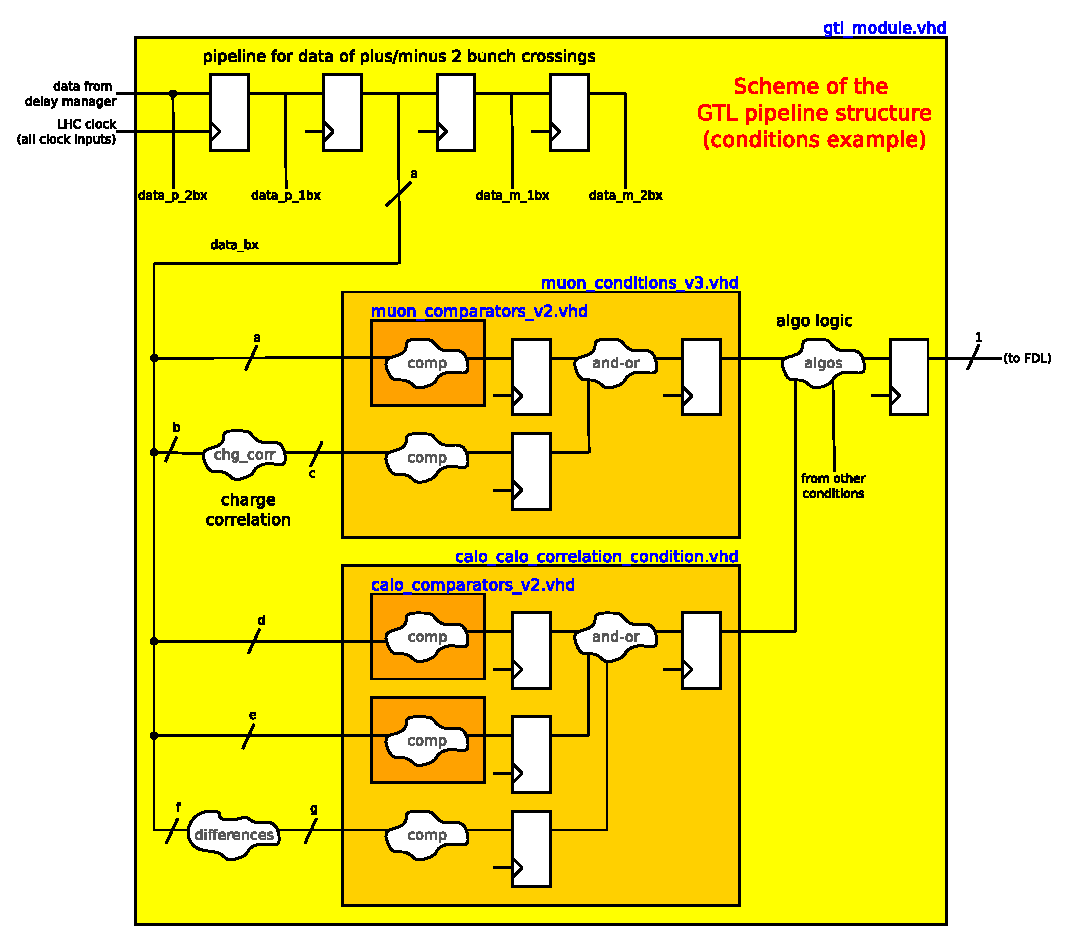
\includegraphics[width=15cm]{figures/gtl_pipeline}
\caption{Scheme of \ugtl pipeline structure}
\label{fig:gtl:gtl_pipeline}
\end{figure}


\subsubsection{Definitions of Calorimeter data}
\label{sec:gtl:calorimeter_data}

The calorimeter trigger processing identifies \textbf{\egamma, jet} and \textbf{tau} objects and \textbf{\esums}.\\
See also \ref{sec:gtl:optical_interfaces}.\\

\textbf{\Egamma}:\\ Twelve objects are passed to the \ugt for each event.\\
For each selected object, the Calo-Layer2 sends parameters for \pt and for position and isolation - encoded in 32 bits:
\begin{itemize}
\item 9 bits \pt, range = 0..255 GeV (HW index = 0..0x1FF), step = 0.5, the highest bin will mark an overflow (HW index 0x1FF): meaning has to be defined
\item 8 (7+1 sign) bits pseudo-rapidity ($\eta$) position, range = -5.0 to 5.0, step = 0.087/2, linear scale, 230 bins (HW index = 0x8E..0x72)
\item 8 bits azimuth angle ($\varphi$) position, range = 2$\pi$, step $\approx$ 2$\pi$/144 (\^=2.5°), 144 bins (HW index = 0..0x8F), HW index starting at 0° (anti-clockwise)
\item 2 bits isolation
\item 5 bits spare
\end{itemize}

\textbf{Jet}:\\ Twelve objects are passed to the \ugt for each event.\\
For each selected object, the Calo-Layer2 sends parameters: \pt, for position information, a DISP bit and quality information - encoded in 32 bits:
\begin{itemize}
\item 11 bits \pt, range = 0..1023 GeV (HW index = 0..0x7FF), step = 0.5, the highest bin will mark an overflow (HW index 0x7FF): meaning has to be defined
\item 8 (7+1 sign) bits pseudo-rapidity ($\eta$) position, range = -5.0 to 5.0, step = 0.087/2, linear scale, 230 bins (HW index = 0x8E..0x72)
\item 8 bits azimuth angle ($\varphi$) position, range = 2$\pi$, step $\approx$ 2$\pi$/144 (\^=2.5°), 144 bins (HW index = 0..0x8F), HW index starting at 0° (anti-clockwise)
\item 1 DISP bit (will be used to flag a jet as delayed / displaced based on HCAL timing and depth profiles that are indicative of a "long lived particle" (LLP) decay. If this bit is set to 1, then the jet has been tagged as a LLP jet.)
\item 2 bits for "quality flags" - currently not used.
\item 2 bits spare
\end{itemize}

\textbf{Tau}:\\ Twelve objects are passed to the \ugt for each event.\\
For each selected object, the Calo-Layer2 sends parameters for \pt and for position information and isolation - encoded in 32 bits:
\begin{itemize}
\item 9 bits \pt, range = 0..255 GeV (HW index = 0..0x1FF), step = 0.5, the highest bin will mark an overflow (HW index 0x1FF): meaning has to be defined
\item 8 (7+1 sign) bits pseudo-rapidity ($\eta$) position, range = -5.0 to 5.0, step = 0.087/2, linear scale, 230 bins (HW index = 0x8E..0x72)
\item 8 bits azimuth angle ($\varphi$) position, range = 2$\pi$, step $\approx$ 2$\pi$/144 (\^=2.5°), 144 bins (HW index = 0..0x8F), HW index starting at 0° (anti-clockwise)
\item 2 bits isolation
\item 5 bits spare
\end{itemize}

The representation of the 8 bits (called "hardware index [HW index]") in $\eta$ is expected as Two's Complement notation as shown below.\\

\begin{table}[ht]
\caption{$\eta$ scale of calorimeter objects}
\vspace{5mm}
\centering
\begin{tabular}{|c|l|c|}\hline
\textbf{HW index}& \textbf{$\eta$ range} & \textbf{$\eta$ bin}\\\hline\hline
0x72 & 114$*$0.087/2 to 115$*$0.087/2 & 114\\\hline
... & ... & ...\\\hline
0x01 & 0.087/2 to 2$*$0.087/2 & 1\\\hline
0x00 & 0 to 0.087/2 & 0\\\hline
0xFF & 0 to -0.087/2 & -1\\\hline
0xFE & -0.087/2 to -2$*$0.087/2 & -2\\\hline
... & ... & ...\\\hline
0x8E & -114$*$0.087/2 to -115$*$0.087/2 & -115\\\hline
\end{tabular}
\label{tab:gtl:calo_eta_scale_new}
\end{table}

The representation of the 8 bits in $\varphi$ is expected as shown in Table~\ref{tab:gtl:calo_phi_scale}.\\

\begin{table}[ht]
\caption{$\varphi$ scale of calorimeter objects}
\vspace{5mm}
\centering
\begin{tabular}{|c|l|l|c|}\hline
HW index & $\varphi$ range & $\varphi$ range [degrees] & $\varphi$ bin\\\hline\hline
0x00 & 0 to 2$\pi$/144 & 0 to 2.5 & 0\\\hline
0x01 & 2$\pi$/144 to 2$*$2$\pi$/144 & 2.5 to 5.0 & 1\\\hline
... & ... & ... & ...\\\hline
0x8F & 143$*$2$\pi$/144 to 2$\pi$ & 357.5 to 360 & 143\\\hline
\end{tabular}
\label{tab:gtl:calo_phi_scale}
\end{table}

The representation of the two bits for isolation (e/$\gamma$ and tau) is expected as shown in Table~\ref{tab:gtl:eg_tau_iso_bits}.\\

\begin{table}[ht]
\caption{Definition of e/$\gamma$ and tau isolation bits}
\vspace{5mm}
\centering
\begin{tabular}{|c|c|}\hline
bits [26..25] & definition \\\hline\hline
00 & not isolated \\
01 & isolated \\
10 & TBD \\
11 & TBD \\\hline
\end{tabular}
\label{tab:gtl:eg_tau_iso_bits}
\end{table}

\clearpage

\subsubsection{Definitions of Energy sum quantities data}

See \ref{sec:gtl:optical_interfaces} for data structure.\\
{\Esums} consist of following quantities (for naming convention see \ref{sec:glossary}):
\begin{itemize}
\item {\ett}
\item {\htt}
\item {\etm}
\item {\htm}
\item {ETTEM}
\item {ET$_{miss}^{HF}$}
\item {HT$_{miss}^{HF}$}
\item {ASYMET}
\item {ASYMHT}
\item {ASYMETHF}
\item {ASYMHTHF}
\item {CENT[0..7]}
\end{itemize}

Calo-Layer2 sends 6 frames (each 32 bits) with Energy sum quantities containing the following information:
\begin{itemize}
\item \et, 12 bits, range = 0..2047 GeV (HW index = 0..0xFFF), step = 0.5, the highest bin will mark an overflow (HW index 0xFFF): meaning has to be defined
\item azimuth angle ($\varphi$) position, 8 bits, range = 2$\pi$, step $\approx$ 2$\pi$/144 (\^=2.5°), 144 bins (HW index = 0..0x8F), HW index starting at 0° (anti-clockwise)
\item "Towercount", 13 bits, range = 0..8191
\item "Minimum bias", 4 bits, range = 0..15
\item "Asymmetry", 8 bits, range = 0..255 (used 0..100)
\item "Centrality", 8 single bits, used as signals
\end{itemize}

Frame 0: The data structure of "Total Et" (\ett) quantity [including "Total Et from ECAL only" (ETTEM) and "minimum bias HF+ threshold 0" bits].

Frame 1: The data structure of "Total calibrated Et in jets" (\htt) quantity [including "towercount" and "minimum bias HF- threshold 0" bits].

Frame 2: The data structure of "Missing Et" (\etm) quantity [including "Asymmetry" ASYMET and "minimum bias HF+ threshold 1" bits].

Frame 3: The data structure of "Missing Ht" (\htm) quantity [including "Asymmetry" ASYMHT and "minimum bias HF- threshold 1" bits].

Frame 4: The data structure of "Missing Et including HF" (ET$_{miss}^{HF}$) quantity [including "Asymmetry" ASYMETHF and "Centrality" bits (3:0)].

Frame 5: The data structure of "Missing Ht including HF" (HT$_{miss}^{HF}$) quantity [including "Asymmetry" ASYMHTHF and "Centrality" bits (7:4)].

\clearpage

\subsubsection{Definitions of Muon data}
\label{sec:gtl:muon_data}
Eight Muon objects are provided by \gmt. One Muon object has a 64 bits data structure with parameters for \pt, for unconstrained \pt, for impact parameter, for position, charge, quality and isolation information (see also \ref{sec:gtl:gmt_optical_interfaces}):\\
\begin{itemize}
\item 10 bits azimuth angle ($\varphi$) position, range = 2$\pi$, step $\approx$ 2$\pi$/576 (\^=0.625°), 576 bins (HW index = 0..0x23F), HW index starting at 0° (anti-clockwise)
\item 9 bits \pt, range = 0..255 GeV (HW index = 0..0x1FF), step = 0.5, the highest bin will mark an overflow (HW index 0x1FF): meaning has to be defined
\item 4 bits quality, 16 types for quality (meaning not defined yet!)
\item 9 (8+1 sign) bits pseudo-rapidity ($\eta$) position, range = -2.45 to 2.45, step = 0.087/8, linear scale, 451 bins (-225..225, HW index = 0x11F..0x0E1)
\item 2 bits isolation, 4 types for isolation (meaning not defined yet!)
\item 1 bit charge sign, charge sign = '0' means "positive" charge, charge sign = '1' means "negative" charge
\item 1 bit charge valid (='1' means "valid")
\item 7 index bits
\item 10 bits azimuth angle ($\varphi$) position, raw data
\item 8 bits unconstrained \pt, range = 0..255 GeV (HW index = 0..0xFF), step = 1.0, the highest bin will mark an overflow (HW index 0xFF)
\item 1 hadronic (muon) shower bit
\item 2 bits impact parameter
\end{itemize}

The representation of the 9 bits (called "hardware index [HW index]") in $\eta$ is expected as Two's Complement notation as shown in Table~\ref{tab:gtl:muon_eta_scale}.\\
The central value of the bin 0 (-0.010875/2 to +0.010875/2) = 0.0, the left edge of the bins will range from $-255 \times 0.010875 - 0.010875/2 = -2.7785625$ to $+255 \times 0.010875 - 0.010875/2 = 2.7676875$.
The central value of the bins will range between $\pm 2.773125$ . The physical $\eta$ range of the muon detectors is about $\pm2.45$, so that not all possible $\eta$ bins will be used.\\

\begin{table}
\caption{$\eta$ scale of muon objects}
\vspace{5mm}
\centering
\begin{tabular}{|c|l|c|}\hline
HW index & $\eta$ range & $\eta$ bin\\\hline\hline
0x0E1 & 224.5$*$0.087/8 to 225.5$*$0.087/8 & 225\\\hline
0x0E0 & 223.5$*$0.087/8 to 224.5$*$0.087/8 & 224\\\hline
... & ... & ...\\\hline
0x001 & 0.5$*$0.087/8 to 1.5$*$0.087/8 & 1\\\hline
0x000 & 0.5$*$-0.087/8 to 0.5$*$0.087/8 & 0\\\hline
0x1FF & 0.5$*$-0.087/8 to 1.5$*$-0.087/8 & -1\\\hline
0x1FE & 1.5$*$-0.087/8 to -2.5$*$0.087/8 & -2\\\hline
... & ... & ...\\\hline
0x11F & -224.5$*$0.087/8 to -225.5$*$0.087/8 & -225\\\hline
\end{tabular}
\label{tab:gtl:muon_eta_scale}
\end{table}

The representation of the 10 bits in $\varphi$ is expected as shown in Table~\ref{tab:gtl:muon_phi_scale}.\\

\begin{table}[ht]
\caption{$\varphi$ scale of muon objects}
\vspace{5mm}
\centering
\begin{tabular}{|c|l|l|c|}\hline
HW index & $\varphi$ range & $\varphi$ range [degrees] & $\varphi$ bin\\\hline\hline
0x000 & 0 to 2$\pi$/576 & 0 to 0.625 & 0\\\hline
0x001 & 2$\pi$/576 to 2$*$2$\pi$/576 & 0.625 to 1.250 & 1\\\hline
... & ... & ... & ...\\\hline
0x23F & 575$*$2$\pi$/576 to 2$\pi$ & 359.375 to 360 & 575\\\hline
\end{tabular}
\label{tab:gtl:muon_phi_scale}
\end{table}

The representation of the four bits for quality is expected as shown in Table~\ref{tab:gtl:muon_quality_bits}.\\

\begin{table}[ht]
\caption{Definition of muon quality bits}
\vspace{5mm}
\centering
\begin{tabular}{|c|c|}\hline
bits [22..19] & definition \\\hline\hline
0000 & quality "level 0" \\
0001 & quality "level 1" \\
... & ... \\
1110 & quality "level 14" \\
1111 & quality "level 15" \\\hline
\end{tabular}
\label{tab:gtl:muon_quality_bits}
\end{table}

\clearpage

The representation of the two bits for isolation is expected as shown in Table~\ref{tab:gtl:muon_iso_bits}.\\

\begin{table}[ht]
\caption{Definition of muon isolation bits}
\vspace{5mm}
\centering
\begin{tabular}{|c|c|}\hline
bits [33..32] & definition \\\hline\hline
00 & not isolated \\
01 & isolated \\
10 & TBD \\
11 & TBD \\\hline
\end{tabular}
\label{tab:gtl:muon_iso_bits}
\end{table}

The representation of the two bits for charge is expected as shown in Table~\ref{tab:gtl:muon_charge_bits}.\\

\begin{table}[ht]
\caption{Definition of muon charge bits}
\vspace{5mm}
\centering
\begin{tabular}{|c|c|}\hline
bits [35..34] & definition \\\hline\hline
00 & not valid charge \\
01 & not valid charge \\
10 & positive charge \\
11 & negative charge \\\hline
\end{tabular}
\label{tab:gtl:muon_charge_bits}
\end{table}

Muon shower bits definition is shown in Table~\ref{tab:gtl:tab_muon_shower_bits}.\\

\begin{table}[ht]
\caption{Definition of hadronic (muon) shower bits on bit 61 of muon objects}
\vspace{5mm}
\centering
\begin{tabular}{|c|c|}\hline
object & definition \\\hline\hline
0 & MUS0 \\
2 & MUS1 \\
4 & MUSOOT0 \\
6 & MUSOOT1 \\\hline
\end{tabular}
\label{tab:gtl:tab_muon_shower_bits}
\end{table}


The representation of the two bits for impact parameter is expected as shown in Table~\ref{tab:gtl:muon_ip_bits}.\\

\begin{table}[ht]
\caption{Definition of muon impact parameter bits}
\vspace{5mm}
\centering
\begin{tabular}{|c|c|}\hline
bits [63..62] & definition \\\hline\hline
00 & TBD \\
01 & TBD \\
10 & TBD \\
11 & TBD \\\hline
\end{tabular}
\label{tab:gtl:muon_ip_bits}
\end{table}

\clearpage

\subsubsection{Calculation of object cuts}
\label{sec:gtl:calc_obj_cuts}

List of object cuts:
\begin{itemize}
\item \pt
\item $\eta$
\item $\varphi$
\item isolation
\item DISP (displaced = "long lived particle" jet)
\item charge
\item quality
\item unconstrained \pt
\item impact parameter
\end{itemize}

\paragraph{Object cuts}
\label{sec:gtl:object_cuts}
The comparisons for objects cuts are done by:\\
A comparator between the energy (\pt) and a threshold (pt\_threshold) with 'mode-selection'. Similar for unconstrained \pt.\\
The comparison in $\eta$ is done with five "window"-comparators, so one gets max. five ranges for $\eta$. The $\eta$ value (HW index) has a Two's Complement notation, the comparisons is done signed. Number of windows is given for $\eta$.\\
The comparison in $\varphi$ is done with two "window"-comparators, so one gets two ranges for $\varphi$. The comparisons is done unsigned. Number of windows is given for $\varphi$.\\
There are two cases how the limits of one "window"-comparator could be set (see also Figure~\ref{fig:gtl:phi_windows_comparator}):
\begin{itemize}
\item Upper limit is less than lower limit => $\varphi$ range between the limits, including the $\varphi$ bin with value = 0 (HW index).
\item Upper limit is greater/equal than lower limit => $\varphi$ range between the limits, not including the $\varphi$ bin with value = 0 (HW index).
\end{itemize}
% \begin{lstlisting}[label=lst:gtl:phi_window_comparator_vhd,float=here,caption=VHDL code of "window"-comparator in $\varphi$,captionpos=t]
\begin{lstlisting}
    phi_comp_w1 <= '1' when phi_w1_upper_limit < phi_w1_lower_limit and
                    (phi <= phi_w1_upper_limit or phi >= phi_w1_lower_limit) else
                   '1' when phi_w1_upper_limit >= phi_w1_lower_limit and
                    (phi <= phi_w1_upper_limit and phi >= phi_w1_lower_limit)
                    else '0';
\end{lstlisting}
Only one of the required ranges ("windows") must be fulfilled by $\eta$ and $\varphi$ values ("or").\\

\clearpage

The comparisons for isolation, quality and impact parameter are done with LUTs.\\
The comparison for charge is done with requested charge.\\
If DISP bit is set to 1, then the jet has been tagged as a "long lived particle" (LLP) jet. A one bit requirement is given for DISP for comparison.\\

\begin{figure}[htb]
\centering
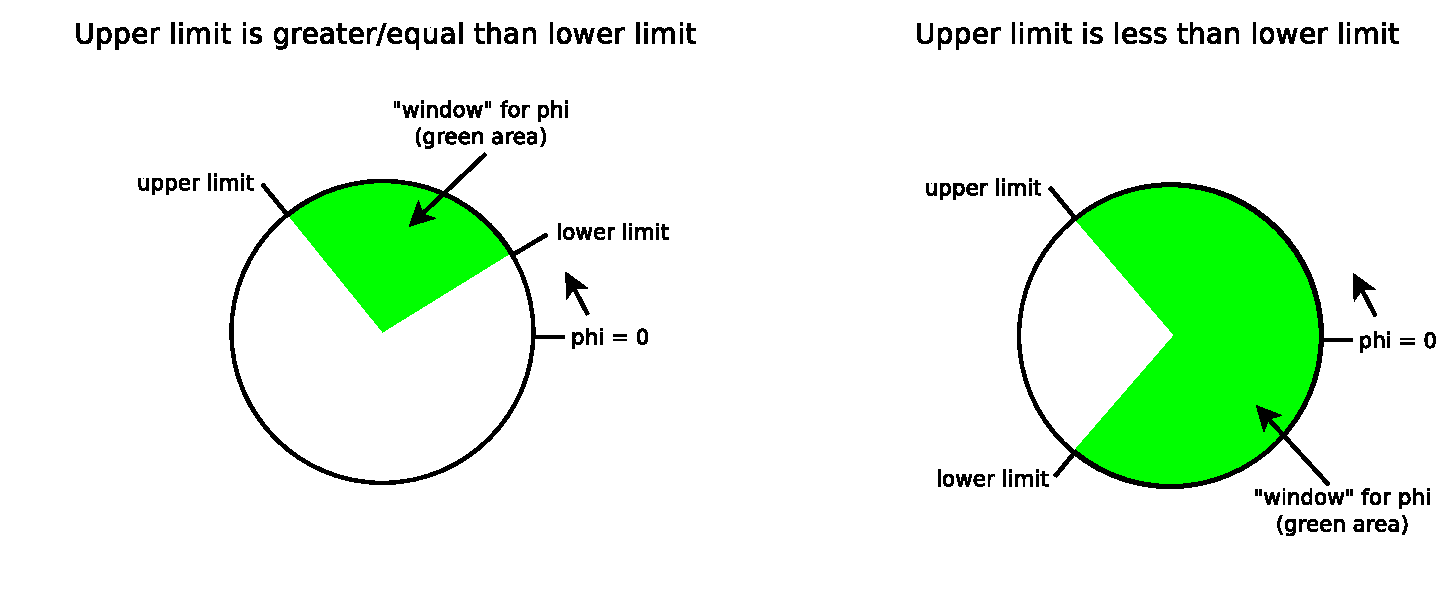
\includegraphics[width=15cm]{figures/phi_windows_comparator}
\caption{Setting the limits for "window"-comparators for $\varphi$}
\label{fig:gtl:phi_windows_comparator}
\end{figure}

The comparison of isolation (for \egamma, tau and muon) is done with a LUT (Table~\ref{tab:gtl:lut_iso}). [To ignore quality comparison, all bits in the LUT have to be '1'.]

\begin{table}[ht]
\caption{LUT contents for isolation comparison}
\vspace{5mm}
\centering
\begin{tabular}{|c|c|p{.4\columnwidth}|}\hline
LUT content (4 bits) & isolation (2 bits) & trigger \\\hline\hline
X"0" & xx & no trigger\\\hline
X"1" & 00 & trigger on isolation bits = 00\\\hline
X"2" & 01 & trigger on isolation bits = 01\\\hline
X"3" & 00 or 01 & trigger on isolation bits = 00 or 01\\\hline
X"4" & 10 & trigger on isolation bits = 10\\\hline
X"5" & 00 or 10 & trigger on isolation bits = 00 or 10\\\hline
X"6" & 01 or 10 & trigger on isolation bits = 01 or 10\\\hline
X"7" & 00 or 01 or 10 & trigger on isolation bits = 00 or 01 or 10\\\hline
X"8" & 11 & trigger on isolation bits = 11\\\hline
X"9" & 00 or 11 & trigger on isolation bits = 00 or 11\\\hline
X"A" & 01 or 11 & trigger on isolation bits = 01 or 11\\\hline
X"B" & 00 or 01 or 11 & trigger on isolation bits = 00 or 01 or 11\\\hline
X"C" & 10 or 11 & trigger on isolation bits = 10 or 11\\\hline
X"D" & 00 or 10 or 11 & trigger on isolation bits = 00 or 10 or 11\\\hline
X"E" & 01 or 10 or 11 & trigger on isolation bits = 01 or 10 or 11\\\hline
X"F" & 00 or 01 or 10 or 11 & trigger on isolation bits = 00 or 01 or 10 or 11 (= "ignore" isolation)\\\hline
\end{tabular}
\label{tab:gtl:lut_iso}
\end{table}

The comparison of impact parameter is done with LUT (Table~\ref{tab:gtl:muon_lut_ip}). [To ignore quality comparison, all bits in the LUT have to be '1'.]

\begin{table}
\caption{LUT contents for impact parameter comparison}
\vspace{5mm}
\centering
\begin{tabular}{|c|c|p{.4\columnwidth}|}\hline
LUT content (4 bits) & impact parameter  (2 bits) & trigger \\\hline\hline
X"0" & xx & no trigger\\\hline
X"1" & 00 & trigger on impact parameter bits = 00\\\hline
X"2" & 01 & trigger on impact parameter bits = 01\\\hline
X"3" & 00 or 01 & trigger on impact parameter bits = 00 or 01\\\hline
X"4" & 10 & trigger on impact parameter bits = 10\\\hline
X"5" & 00 or 10 & trigger on impact parameter bits = 00 or 10\\\hline
X"6" & 01 or 10 & trigger on impact parameter bits = 01 or 10\\\hline
X"7" & 00 or 01 or 10 & trigger on impact parameter bits = 00 or 01 or 10\\\hline
X"8" & 11 & trigger on impact parameter bits = 11\\\hline
X"9" & 00 or 11 & trigger on impact parameter bits = 00 or 11\\\hline
X"A" & 01 or 11 & trigger on impact parameter bits = 01 or 11\\\hline
X"B" & 00 or 01 or 11 & trigger on impact parameter bits = 00 or 01 or 11\\\hline
X"C" & 10 or 11 & trigger on impact parameter bits = 10 or 11\\\hline
X"D" & 00 or 10 or 11 & trigger on impact parameter bits = 00 or 10 or 11\\\hline
X"E" & 01 or 10 or 11 & trigger on impact parameter bits = 01 or 10 or 11\\\hline
X"F" & 00 or 01 or 10 or 11 & trigger on impact parameter bits = 00 or 01 or 10 or 11 (= "ignore" impact parameter)\\\hline
\end{tabular}
\label{tab:gtl:muon_lut_ip}
\end{table}

The comparison of quality is done with LUT (Table~\ref{tab:gtl:muon_lut_qual}). [To ignore quality comparison, all bits in the LUT have to be '1'.]

\begin{table}
\caption{LUT contents for quality comparison of muon objects}
\vspace{5mm}
\centering
\begin{tabular}{|c|c|l|c|}\hline
LUT content (16 bits) & quality bits  (4 bits) & trigger \\\hline\hline
X"0000" & xxxx & no trigger\\\hline
X"0001" & 0000 & trigger on quality "level 0"\\\hline
X"0002" & 0001 & trigger on quality "level 1"\\\hline
X"0003" & 0001 or 0000 & trigger on quality "level 1" or "level 0"\\\hline
X"0004" & 0010 & trigger on quality "level 2"\\\hline
... & ...& ...\\\hline
X"8000" & 1111 & trigger on quality "level 15"\\\hline
X"C000" & 1111 or 1110 & trigger on quality "level 15" or "level 14"\\\hline
... & ...& ...\\\hline
X"FFFF" & xx & trigger on all quality "levels" (= "ignore")\\\hline
\end{tabular}
\label{tab:gtl:muon_lut_qual}
\end{table}

Charge valid and charge sign bits must be equal to the requested charge.\\

\clearpage

\subsubsection{Calculation of correlation cuts}
\label{sec:gtl:calc_corr_cuts}

The following cuts are used for two objects correlations:
\begin{itemize}
\item $\Delta\eta$ (DETA).
\item $\Delta\varphi$ (DPHI).
\item $\Delta$R (DR).
\item charge correlation (only for muon).
\item Cuts for mass (MASS) of following mass types:
  \begin{itemize}
  \item Invariant mass.
  \item Invariant mass with unconstrained pt (for muons only).
  \item Invariant mass over $\Delta$R.
  \item Transverse mass.
  \end{itemize}
\item Two-body pt.
\end{itemize}
There is one mass cut for correlations with three objects:
\begin{itemize}
\item Invariant mass for three objects (MASS).
\end{itemize}

The generation of look-up-tables (LUTs) for calculations of correlation cuts is described in chapter "Calculation of look-up-tables (LUTs) for correlation cuts" (see \ref{sec:gtl:calc_luts_corr_cuts}).

\paragraph{Calculation of $\Delta\eta$}
\label{sec:gtl:calculation_delta_eta}

The calculation of \textit{$\Delta\eta$} of two objects is done with formula:

$\Delta\eta$=abs($\eta$1-$\eta$2)

where $\eta$1 and $\eta$2 are represented in signed hardware indices.

% LUTs are used to provide $\Delta\eta$ values for comparison in VHDL with requirements, given by TME and VHDL Producer as two thresholds: "greater/equal lower limit" and "less/equal upper limit".

\paragraph{Calculation of $\Delta\varphi$}
\label{sec:gtl:calculation_delta_phi}

The calculation of \textit{$\Delta\varphi$} of two objects is done with formula:

$\Delta\varphi$=abs($\varphi$1-$\varphi$2) with ("$\varphi$ full bin range"-$\Delta\varphi$) when ($\Delta\varphi$ > "$\varphi$ half bin range").

where $\varphi$1 and $\varphi$2 are represented in unsigned hardware indices.

\paragraph{$\Delta$R calculation}
\label{sec:gtl:delta_r_calculation}

The calculation of \textit{$\Delta$R} of two objects is done with formula:

$\Delta$R=$\sqrt{(\eta1-\eta2)^2+(\varphi1-\varphi2)^2}$.

The calculation of $\Delta$$R^2$ in VHDL (no square root in VHDL) is done by adding the square of $\Delta\eta$ and $\Delta\varphi$ LUT values.

\paragraph{Invariant mass calculation}
\label{sec:gtl:inv_mass_calculation}

The calculation of \textit{invariant mass of two objects} is done with formula:

M=$\sqrt{2 pt_1  pt_2 (\cosh(\eta1-\eta2)-\cos(\varphi1-\varphi2))}$.

The calculation of $\frac{M^2}{2}$ in VHDL (no square root in VHDL) is done by multiplying LUT values of pt1, pt2 and the difference of $\cosh($$\Delta\eta$$)$ and $\cos($$\Delta\varphi$$)$.

\paragraph{Transverse mass calculation}
\label{sec:gtl:transverse_mass_calculation}

The calculation of \textit{transverse mass of two objects} is done with formula:

M=$\sqrt{2 pt_1 pt_2 (1-\cos(\varphi1-\varphi2))}$.

Calculation similar to "Invariant mass calculation".

\paragraph{Invariant mass over $\Delta$R calculation}
\label{sec:gtl:inv_mass_div_dr_calculation}

The formulas for \textit{invariant mass over $\Delta$R of two objects} are:

M=$\sqrt{2 pt_1  pt_2 (\cosh(\eta1-\eta2)-\cos(\varphi1-\varphi2))}$.

$\Delta$R=$\sqrt{(\eta1-\eta2)^2+(\varphi1-\varphi2)^2}$.

% In the TME there is one threshold for M/$\Delta$R, given in GeV (floating point notation) with one position after decimal point.
The calculation of \textit{invariant mass over $\Delta$R of two objects} is done with $\frac{M^2}{2}\times$(1/$\Delta$$R^2$) (no square root in VHDL).\\
A direct calculation of 1/$\Delta$$R^2$ is not possible in firmware (VHDL code), therefore the implementation of the calculation is done by LUTs. In the hardware the values of these LUTs are stored in "large" ROMs, which was realized using the Block RAMs (BRAMs) of the Virtex chip.\\
Due the limited number of available BRAMs there are some restrictions for creating algorithms with \textit{invariant mass over $\Delta$R}:
\begin{itemize}
\item Objects must have the same type (e.g.: "muon muon", "eg eg", ...)
\item Objects must be of same bx
\item Resolution of $\Delta\eta$ and $\Delta\varphi$:
  \begin{itemize}
  \item Full resolution for calos (max. deta bins=230, max. dphi bins=72)
  \item Half resolution only for muons (max. deta bins=226, max. dphi bins=144)
  \end{itemize}
\item If 1/$\Delta$$R^2$=0 ($\Delta\eta$=0 and $\Delta\varphi$=0) then correlation cut \textit{invariant mass over $\Delta$R} is true
\item The values of LUTs are only valid for current definitions and restrictions. Every change might cause a recalculation of the values and a regeneration of IPs (representing LUTs in BRAMs) in Vivado (firmware generation tool)
\end{itemize}

The values of LUTs in firmware are listed in coe files of ROMs (created by same scripts mentioned above), currently 5 ROMs for "calo calo" and 6 ROMs for "muon muon" (see \href{\gitbranch/firmware/ngc/blk_mem_gen_v8_4_4/lut_calo_inv_dr_sq_rom1.coe}{\texttt{\textquotesingle lut\_calo\_inv\_dr\_sq\_rom1.coe\textquotesingle }}, etc. and \href{\gitbranch/firmware/ngc/blk_mem_gen_v8_4_4/lut_muon_inv_dr_sq_rom1.coe}{\texttt{\textquotesingle lut\_muon\_inv\_dr\_sq\_rom1.coe\textquotesingle }}, etc.). The addresses of the BRAMs are given by $\Delta\eta$ and $\Delta\varphi$. All ROMs for calos have 4096 addresses, for muons 8192 addresses. The data width of ROMs is different depending on the highest LUT value in ROM. Because of these different data widths, the partitioning of several ROMs was done to save BRAM resources. Currently 873 BRAMs (36kb) are available per Virtex chip.
Following numbers of BRAMs (36kb) are needed for:
\begin{itemize}
\item "calo calo": 660
\item "muon muon": 672
\end{itemize}
Currently one calculation of \textit{invariant mass over $\Delta$R} of "calo calo" or "muon muon" is possible in one Virtex chip, but one can have some algorithms containing \textit{invariant mass over $\Delta$R} with different thresholds, but with same objects and same bx.

\paragraph{Invariant mass calculation for three objects}
\label{sec:gtl:inv_mass_3_obj_calculation}

The calculation of \textit{invariant mass calculation for three objects} is done by calculating the invariant mass for all two-object combinations and take the sum of the three invariant masses of the two-object combinations.
% In the TME there are two thresholds for M: "greater/equal lower limit" and "less/equal upper limit", given in GeV (floating point notation) with one position after decimal point in even numbers.

\paragraph{Two-body pt calculation}
\label{sec:gtl:twobody_pt_calculation}

The calculation of \textit{two-body pt} is done with formula:\\

pt=$\sqrt{pt^2_1 + pt^2_2 + 2  pt_1 pt_2 (\cos(\varphi1) \cos(\varphi2) + \sin(\varphi1) \sin(\varphi2))}$\\

The calculation of ${pt^2}$ in VHDL (no square root in VHDL) using LUTs for pt1, pt2, $\cos($$\varphi$$)$ and $\sin($$\varphi$$)$.

% In the TME there is one threshold for pt, given in GeV (floating point notation) with one position after decimal point.
% The comparison in VHDL is done with ${pt^2}$ (no square root in VHDL), threshold for ${pt^2}$ is provided by VHDL-Producer.

\paragraph{Muon charge correlation}
\label{sec:gtl:muon_charge_correlation_module}

For definition of muon charge, see \ref{sec:gtl:muon_data}.\\
In the muon charge correlation module (\href{\gitbranch/firmware/hdl/gt_mp7_core/gtl_fdl_wrapper/gtl/muon_charge_correlations.vhd}{\texttt{\textquotesingle muon\_charge\_correlations.vhd\textquotesingle }}), the charge correlations are made for different muon conditions types. The module is instantiated in the top-of-hierarchy module (\href{\gitbranch/firmware/hdl/payload/gtl\_module\_tpl.vhd}{\texttt{\textquotesingle gtl\_module.vhd\textquotesingle }})
and not inside of a muon conditions module.
The charges of objects (number of objects depends on muon condition type) are compared to get "like sign charge" ("LS") or "opposite sign charge" ("0S"), "LS" means that the charges (charge sign)
of objects are the same, "0S" means that at least one object has different charge than the others. This information is used in all instatiated muon conditions.
There is no charge correlation for single type conditions.\\
In all cases the "charge valid" bit of the objects must be set.\\
In TME one can select "LS", "0S" or ignore for charge correlation in muon conditions.

% \begin{table}[ht]
% \caption{Muon charge correlation - Double Muon}
% \vspace{5mm}
% \centering
% \begin{tabular}{|c|l|}\hline
% \verb|x x| & I ignore (charge x = +, -, I) \\
% \verb|+ +| & LS both positive muons \\
% \verb|- -| & LS both negative muons \\
% \verb|I I| & LS both muons with the same sign, positive or negative \\
% \verb|+ -| & OS two muons of opposite sign \\
% \verb|- +| & OS idem \\
% \verb|I I| & OS idem \\\hline
% \end{tabular}
% \label{tab:gtl:muon_charge_corr_double}
% \end{table}

\begin{table}[ht]
\caption{Muon charge correlation - Double Muon}
\vspace{5mm}
\centering
\begin{tabular}{|c|l|}\hline
\verb|x x| & I ignore (charge x = +, -, I) \\
\verb|+ +| & LS both positive muons \\
\verb|- -| & LS both negative muons \\
\verb|+ -| & OS two muons of opposite sign (a pair) \\
\verb|- +| & OS two muons of opposite sign (a pair) \\\hline
\end{tabular}
\label{tab:gtl:muon_charge_corr_double}
\end{table}

% \begin{table}[ht]
% \caption{Muon charge correlation - Triple Muon}
% \vspace{5mm}
% \centering
% \begin{tabular}{|c|l|}\hline
% \verb|x x x| & I  ignore (charge x = +, -, I) \\
% \verb|+ + +| & LS three muons of positive charge \\
% \verb|- - -| & LS three muons of negative charge \\
% \verb|I I I| & LS three muons of the same sign (positive or negative) \\
% \verb|+ + -| & OS a pair plus a positive muon \\
% \verb|+ - -| & OS a pair plus a negative muon \\
% \verb|+ - I| & OS a pair plus a negative or positive muon \\\hline
% \end{tabular}
% \label{tab:gtl:muon_charge_corr_triple}
% \end{table}

\begin{table}[ht]
\caption{Muon charge correlation - Triple Muon}
\vspace{5mm}
\centering
\begin{tabular}{|c|l|}\hline
\verb|x x x| & I  ignore (charge x = +, -, I) \\
\verb|+ + +| & LS three muons of positive charge \\
\verb|- - -| & LS three muons of negative charge \\
\verb|- + +| & OS a pair plus a positive muon \\
\verb|+ - +| & OS a pair plus a positive muon \\
\verb|+ + -| & OS a pair plus a positive muon \\
\verb|+ - -| & OS a pair plus a negative muon \\
\verb|- + -| & OS a pair plus a negative muon \\
\verb|- - +| & OS a pair plus a negative muon \\\hline
\end{tabular}
\label{tab:gtl:muon_charge_corr_triple}
\end{table}

% \begin{table}[ht]
% \caption{Muon charge correlation - Quad Muon}
% \vspace{5mm}
% \centering
% \begin{tabular}{|c|l|}\hline
% \verb|x x x x| & I  ignore (charge x = +, -, I) \\
% \verb|+ + + +| & LS four muons of positive charge \\
% \verb|- - - -| & LS four muons of negative charge \\
% \verb|I I I I| & LS four muons of the same sign (positive or negative) \\
% \verb|+ + + -| & OS a pair plus two positive muons \\
% \verb|+ + - -| & OS two pairs \\
% \verb|+ - - -| & OS a pair plus two negative muons \\
% \verb|+ - I I| & OS a pair plus two negative or positive muons \\\hline
% \end{tabular}
% \label{tab:gtl:muon_charge_corr_quad}
% \end{table}

\begin{table}[ht]
\caption{Muon charge correlation - Quad Muon}
\vspace{5mm}
\centering
\begin{tabular}{|c|l|}\hline
\verb|x x x x| & I  ignore (charge x = +, -, I) \\
\verb|+ + + +| & LS four muons of positive charge \\
\verb|- - - -| & LS four muons of negative charge \\
\verb|- + + +| & OS a pair plus two positive muons \\
\verb|+ - + +| & OS a pair plus two positive muons \\
\verb|+ + - +| & OS a pair plus two positive muons \\
\verb|+ + + -| & OS a pair plus two positive muons \\
\verb|+ + - -| & OS two pairs \\
\verb|+ - + -| & OS two pairs \\
\verb|+ - - +| & OS two pairs \\
\verb|- - + +| & OS two pairs \\
\verb|- + - +| & OS two pairs \\
\verb|- + + -| & OS two pairs \\
\verb|+ - - -| & OS a pair plus two negative muons \\
\verb|- + - -| & OS a pair plus two negative muons \\
\verb|- - + -| & OS a pair plus two negative muons \\
\verb|- - - +| & OS a pair plus two negative muons \\\hline
\end{tabular}
\label{tab:gtl:muon_charge_corr_quad}
\end{table}

\clearpage

\subsubsection{Calculation of look-up-tables (LUTs) for correlation cuts}
\label{sec:gtl:calc_luts_corr_cuts}

LUTs are defined as a VHDL "constant" in \href{\gitbranch/firmware/hdl/packages/gtl_pkg.vhd}{\texttt{\textquotesingle gtl\_pkg.vhd\textquotesingle }} (VHDL package file).
The values of precision and step size are given by "scale\_set" in XML file of a L1 menu.

Overview of precision types for correlation cuts (an example for \egamma \egamma correlation):
\begin{itemize}
\item \textit{EG-EG-Delta} relevant for DeltaEta and DeltaPhi LUTs
\item \textit{EG-EG-MassPt} relevant for pt and unconstrained pt LUTs (used in mass and two-body pt calculations)
\item \textit{EG-EG-Math} relevant for cos(DeltaPhi) and cosh(DeltaEta) LUTs (used in mass calculations)
\item \textit{EG-EG-InverseDeltaRMath} relevant for 1/DeltaR LUTs (used in mass over deltaR calculations)
\item \textit{EG-EG-TwoBodyPtMath} relevant for cos(Phi) and sin(Phi) LUTs (used in two-body pt calculations)
\item \textit{EG-EG-DeltaOverlapRemoval} is obsolete, used EG-EG-Delta (same scales for $\eta$ and $\varphi$)
\item \textit{EG-EG-Mass} currently not used
\item \textit{EG-EG-TwoBodyPt} is obsolete, used EG-EG-MassPt
\end{itemize}

Overview of precision names (example for "MassPt"):\\
\tiny{EG-EG-MassPt\\
EG-JET-MassPt\\
EG-TAU-MassPt\\
JET-JET-MassPt\\
JET-TAU-MassPt\\
EG-ETM-MassPt\\
JET-ETM-MassPt\\
TAU-ETM-MassPt\\
EG-HTM-MassPt\\
JET-HTM-MassPt\\
TAU-HTM-MassPt\\
EG-ETMHF-MassPt\\
JET-ETMHF-MassPt\\
TAU-ETMHF-MassPt\\
EG-MU-MassPt\\
JET-MU-MassPt\\
TAU-MU-MassPt\\
MU-MU-MassPt\\
MU-ETM-MassPt\\
MU-HTM-MassPt\\
MU-ETMHF-MassPt}\normalsize

\paragraph{LUTs for \pt and unconstrained \pt used in mass and two-body pt calculations}
\label{sec:gtl:calc_luts_pt}

The values of \pt or unconstrained \pt LUT are calculated by building the half difference of maximum and minimum value of a bin, adding minimum value, rounding at precision position after decimal point and multiplying with 10\textsuperscript{\tiny{precision}} to get integer values.\\
The address input of the LUT for \pt or unconstrained \pt is the value of hardware index of \pt or unconstrained \pt.

The precision values in XML file are given by (an example for \egamma \egamma correlation):\\
\textit{<scale>\\
    <object>PRECISION</object>\\
    <type>EG-EG-MassPt</type>\\
    ...\\
    <n\_bits>1</n\_bits>\\
</scale>}\\

VHDL names of \pt and unconstrained \pt LUTs:\\
\tiny{EG\_PT\_LUT (used also for tau)\\
JET\_PT\_LUT\\
ETM\_PT\_LUT (used also for \htm and ET$_{miss}^{HF}$)\\
MU\_PT\_LUT\\
MU\_UPT\_LUT}\normalsize

\paragraph{LUTs for delta eta}
\label{sec:gtl:calc_luts_delta_eta}

The values of the LUT for $\Delta\eta$ are calculated by multiplying $\Delta\eta$ in hardware indices with $\eta$ step size, rounding at precision position after decimal point and multipling the result with 10\textsuperscript{\tiny{precision}} to get integer values.\\
The address of the LUT is the value of $\Delta\eta$ in hardware indices.\\

The precision value in XML file is given by (an example for \egamma \egamma correlation):\\
\textit{<scale>\\
    <object>PRECISION</object>\\
    <type>EG-EG-Delta</type>\\
    ...\\
    <n\_bits>3</n\_bits>\\
</scale>}\\
where <n\_bits> is the precision value and <type> represents a precision name.\\

The $\eta$ (=$\Delta\eta$) step size in XML file is given by (an example for \egamma):\\
\textit{<scale>\\
<object>EG</object>\\
    <type>ETA</type>\\
    ...\\
    <step>+4.3499999999999997E-02</step>\\
...\\
</scale>}\\

VHDL names of $\Delta\eta$ LUTs:\\
\tiny{CALO\_CALO\_DIFF\_ETA\_LUT\\
CALO\_MU\_DIFF\_ETA\_LUT\\
MU\_MU\_DIFF\_ETA\_LUT}\normalsize

\paragraph{LUTs for delta phi}
\label{sec:gtl:calc_luts_delta_phi}

The values of the LUT for $\Delta\varphi$ are calculated by multiplying $\Delta\varphi$ in hardware indices with $\varphi$ step size, rounding at precision position after decimal point and multipling the result with 10\textsuperscript{\tiny{precision}} to get integer values.\\
The address of the LUT is the value of $\Delta\varphi$ in hardware indices.\\

The precision values of $\Delta\varphi$ are identical with $\Delta\eta$.\\

The $\varphi$ (=$\Delta\varphi$) step size in XML file is given by (an example for \egamma):\\
\textit{<object>EG</object>\\
    <type>PHI</type>\\
    ...\\
    <step>+4.3633231299858237E-02</step>\\
...\\
</scale>}\\

VHDL names of $\Delta\varphi$ LUTs:\\
\tiny{CALO\_CALO\_DIFF\_PHI\_LUT\\
CALO\_MU\_DIFF\_PHI\_LUT\\
MU\_MU\_DIFF\_PHI\_LUT}\normalsize

\paragraph{LUTs for cosh(delta eta) used in mass calculations}
\label{sec:gtl:calc_luts_cosh_delta_eta}

The values in the LUT for $\cosh($$\Delta\eta$$)$ are calculated by multiplying $\Delta\eta$ in hardware indices with $\eta$ step size, calculating cosine hyperbolic, rounding at "Math" precision position after decimal point and multipling the result with 10\textsuperscript{\tiny{precision}} to get integer values.\\
The address of the LUT for $\cosh($$\Delta\eta$$)$ is the value of $\Delta\eta$ in hardware indices.\\
For calo muon correlations one has to use the muon step size.\\

The precision values in XML file are given by (an example for \egamma \egamma correlation):\\
\textit{<scale>\\
    <object>PRECISION</object>\\
    <type>EG-EG-Math</type>\\
    ...\\
    <n\_bits>3</n\_bits>\\
</scale>}\\
used for $\cosh($$\Delta\eta$$)$ and $\cos($$\Delta\varphi$$)$.\\

VHDL names of $\cosh($$\Delta\eta$$)$ LUTs:\\
\tiny{CALO\_CALO\_COSH\_DETA\_LUT\\
CALO\_MUON\_COSH\_DETA\_LUT\\
MU\_MU\_COSH\_DETA\_LUT}\normalsize

\paragraph{LUTs for cos(delta phi) used in mass calculations}
\label{sec:gtl:calc_luts_cos_delta_phi}

The values in the LUT for $\cos($$\Delta\varphi$$)$ are calculated by multiplying $\Delta\varphi$ in hardware indices with $\varphi$ step size, calculating cosine, rounding at "Math" precision position after decimal point and multipling the result with 10\textsuperscript{\tiny{precision}} to get integer values.\\
The address of the LUT for $\cos($$\Delta\varphi$$)$ is the value of $\Delta\varphi$ in hardware indices.
For calo muon correlations one has to use the muon step size.\\

VHDL names of $\cos($$\Delta\varphi$$)$ LUTs:\\
\tiny{CALO\_CALO\_COS\_DPHI\_LUT\\
CALO\_MUON\_COS\_DPHI\_LUT\\
MU\_MU\_COS\_DPHI\_LUT}\normalsize

\paragraph{LUTs for 1/deltaR**2 used in mass over deltaR calculations}
\label{sec:gtl:calc_luts_inverse_deltaR}

The calculation of 1/$\Delta$$R^2$ is done by multiplying $\Delta\eta$ in hardware indices with $\eta$ step size, making the square, doing the same for $\Delta\varphi$,
adding the squares, inverting the sum, rounding at "InverseDeltaRMath" precision position after decimal point and multipling the result with 10\textsuperscript{\tiny{precision}} to get integer values.
The address of the two-dimensional LUT for 1/$\Delta$$R^2$ consists of values of $\Delta\eta$ and $\Delta\varphi$ in hardware indices.\\

The precision values in XML file are given by (an example for \egamma \egamma correlation):\\
\textit{<scale>\\
    <object>PRECISION</object>\\
    <type>EG-EG-InverseDeltaRMath</type>\\
    ...\\
    <n\_bits>5</n\_bits>\\
</scale>}\\

Precision names for "InverseDeltaRMath":\\
\tiny{EG-EG-InverseDeltaRMath\\
JET-JET-InverseDeltaRMath\\
TAU-TAU-InverseDeltaRMath\\
MU-MU-InverseDeltaRMath}\normalsize

The LUTs are located in BRAMs.\\
For calo-calo mass over deltaR 5 ROMs are needed to represend the LUT. The content of the LUT one can see in \href{\gitbranch/firmware/hdl/ngc/blk_mem_gen_v8_4_4/lut_calo_inv_dr_sq_rom1.coe}{\texttt{\textquotesingle lut\_calo\_inv\_dr\_sq\_rom1.coe\textquotesingle }} (and so on).\\
For muon-muon mass over deltaR 6 ROMs are needed to represend the LUT. The content of the LUT one can see in \href{\gitbranch/firmware/hdl/ngc/blk_mem_gen_v8_4_4/lut_muon_inv_dr_sq_rom1.coe}{\texttt{\textquotesingle lut\_muon\_inv\_dr\_sq\_rom1.coe\textquotesingle }} (and so on).\\
The access to a certain ROM depends on the values of $\Delta\eta$ and $\Delta\varphi$ (see \href{\gitbranch/test_rom_lut_calo_inv_dr_sq_all/doc/description_rom_lut_calo_inv_dr_sq.txt}{\texttt{\textquotesingle description\_rom\_lut\_calo\_inv\_dr\_sq.txt\textquotesingle }} and \href{\gitbranch/firmware/hdl/payload/gtl/common/rom_lut_calo_inv_dr_sq_all.vhd}{\texttt{\textquotesingle rom\_lut\_calo\_inv\_dr\_sq\_all.vhd\textquotesingle }}, respectively\\
\href{\gitbranch/test_rom_lut_muon_inv_dr_sq_all/doc/description_rom_lut_muon_inv_dr_sq.txt}{\texttt{\textquotesingle description\_rom\_lut\_muon\_inv\_dr\_sq.txt\textquotesingle }} and\\
\href{\gitbranch/firmware/hdl/payload/gtl/common/rom_lut_muon_inv_dr_sq_all.vhd}{\texttt{\textquotesingle rom\_lut\_muon\_inv\_dr\_sq\_all.vhd\textquotesingle }}).\\
The calculation of values for LUTs is done by python script \href{\gitbranch/scripts/rom_one_over_dr_sq/one_over_dr_sq_calc.py}{\texttt{\textquotesingle one\_over\_dr\_sq\_calc.py\textquotesingle }}. Calculated values one can see in \href{\gitbranch/doc/rom_one_over_dr_sq/emulator_lut_calo_one_over_dr_sq_calc.txt}{\texttt{\textquotesingle emulator\_lut\_calo\_one\_over\_dr\_sq\_calc.txt\textquotesingle }} and \href{\gitbranch/doc/rom_one_over_dr_sq/emulator_lut_muon_one_over_dr_sq_calc.txt}{\texttt{\textquotesingle emulator\_lut\_muon\_one\_over\_dr\_sq\_calc.txt\textquotesingle }}.

\paragraph{LUTs for cos(phi) used in two-body pt calculations}
\label{sec:gtl:calc_luts_cos_phi}

The values in the LUT for $\cos($$\varphi$$)$ are calculated by building the half difference of maximum and minimum value of a $\varphi$ bin, adding minimum value, calculating cosine, rounding at "TwoBodyPtMath" precision position after decimal point and multipling the result with 10\textsuperscript{\tiny{precision}} to get integer values.\\

The precision values in XML file are given by (an example for \egamma \egamma correlation):\\
\textit{<scale>\\
    <object>PRECISION</object>\\
    <type>EG-EG-TwoBodyPtMath</type>\\
    ...\\
    <n\_bits>3</n\_bits>\\
</scale>}\\
used for $\cos($$\varphi$$)$ and $\sin($$\varphi$$)$.\\

VHDL names of $\cos($$\varphi$$)$ LUTs:\\
\tiny{CALO\_COS\_PHI\_LUT\\
MUON\_COS\_PHI\_LUT}\normalsize

\paragraph{LUTs for sin(phi) used in two-body pt cuts}
\label{sec:gtl:calc_luts_sin_phi}

The values in the LUT for $\sin($$\varphi$$)$ are calculated by building the half difference of maximum and minimum value of a $\varphi$ bin, adding minimum value, calculating sine, rounding at "TwoBodyPtMath" precision position after decimal point and multipling the result with 10\textsuperscript{\tiny{precision}} to get integer values.\\

VHDL names of $\sin($$\varphi$$)$ LUTs:\\
\tiny{CALO\_SIN\_PHI\_LUT\\
MUON\_SIN\_PHI\_LUT}\normalsize

\clearpage

\subsubsection{Combination conditions}
\label{sec:gtl:combination_conditions}

\paragraph{Combination conditions definition}
\label{sec:gtl:comb_cond_def}

A condition consists of input data and a set of requirements, which contain the requirements to be complied. The requirements are called "object cuts".

The requirement list contains:\\
thresholds for \pt, ranges for $\eta$ and $\varphi$, LUTs for isolation, LUTs for quality, requsted charges, thresholds for unconstrained \pt, a LUT for impact parameter.
The condition is complied, if every comparison between object parameters and requirements is valid for the following object cuts (only for requested cuts):

For Calorimeter input data:
\begin{itemize}
\item \pt greater-equal (or equal) threshold
\item $\eta$ in range
\item $\varphi$ in range
\item iso LUT
\end{itemize}

For Muon input data:
\begin{itemize}
\item \pt greater-equal (or equal) threshold
\item $\eta$ in range
\item $\varphi$ in range
\item iso LUT
\item requested charge
\item quality LUT
\item unconstrained \pt greater-equal (or equal) threshold
\item impact parameter LUT
\end{itemize}

There are different types of conditions implemented, depending of how many objects have to comply the requirements.
\begin{itemize}
\item "Quad objects requirements condition": this condition type consists of requirements for 4 different trigger objects of the same object type.
For each object the requirements can be different. To fulfill this condition, there must exist at least one set of 4 different objects,
each of which fulfills at least one of the requirements.
\item "Triple objects requirements condition": this condition type consists of requirements for 3 different trigger objects of the same object type.
For each object the requirements can be different. To fulfill this condition, there must exist at least one set of 3 different objects,
each of which fulfills at least one of the requirements.
\item "Double objects requirements condition": this condition type consists of requirements for 2 different trigger objects of the same object type.
For each object the requirements can be different. To fulfill this condition, there must exist at least one set of 2 different objects,
each of which fulfills at least one of the requirements.\footnote{"Double objects requirements condition with spatial correlation" not used anymore, replaced by Correlation conditions}
\item "Single object requirement condition": this condition type consists of one requirement for one trigger object of a given object type.
To fulfill this condition, there must exist at least one object which fulfills the requirement.
\end{itemize}

The values of the requirements are given by VHDL Producer for every Trigger Menu.\\
The input data objects have to be of same type and same bunch-crossing.

With "Double objects requirements condition" a correlation cut of "two-body pt" can be required (calorimeter and muon objects).\\
Additionally charge correlation cuts with "Double objects requirements condition", "Triple objects requirements condition" and "Quad objects requirements condition" of muon objects can be required.

\clearpage

\subsubsection{Energy sum quantities conditions}
\label{sec:gtl:esums_conditions}

\paragraph{Energy sum quantities conditions module (including Asymmetry conditions)}

A comparator between \et and a threshold (et\_threshold) and, depending on object type, a comparison in $\varphi$ with
two "window"-comparators is done in this module.
The value for \et threshold, the \textquotesingle mode-selection\textquotesingle\  for the \et comparator and the limits for the "window"-comparators are given in the generic interface list of the module.
The selection whether a comparison in $\varphi$ is part of the condition is done with the value of the generic parameter \textquotesingle obj\_type\textquotesingle\
(\textquotesingle ETM\_TYPE\textquotesingle\ , \textquotesingle ETMHF\_TYPE\textquotesingle\ , \textquotesingle HTM\_TYPE\textquotesingle\ and \textquotesingle HTMHF\_TYPE\textquotesingle\ force a comparison).
The comparison in $\varphi$ is done in the same way as for calorimeter conditions.
Additionally the data structure of input data (data\_i in port interface list) is provided
as a record in this list. The output signal of the module is in high state, if all comparisons are true.\\
Data for Asymmetry trigger are received on 4 frames on bits 27..20 (8 bits). For every type a comparision with an 8-bit threshold (greater-equal [or equal]) is done.
Asymmetry data are interpreted as counts.\\
For the entity declaration of \href{\gitbranch/firmware/hdl/gt_mp7_core/gtl_fdl_wrapper/gtl/esums_conditions.vhd}{\texttt{\textquotesingle esums\_conditions.vhd\textquotesingle }}, see Listing~\ref{lst:gtl:esums_conditions_vhd}.

\clearpage

\lstinputlisting[label=lst:gtl:esums_conditions_vhd,language=VHDL,caption=Entity declaration of \texttt{esums\_conditions.vhd}]{interfaces/esums_conditions.vhd}

\medskip
\begin{table}
\footnotesize
\caption{Explanation of Listing~\ref{lst:gtl:esums_conditions_vhd}}
\vspace{5mm}
\centering
\begin{tabular}{l p{.7\columnwidth}}
\toprule
{Item} & {Explanation}\\
\midrule
\verb|et_ge_mode| & "mode-selection" for the \et comparator. Valid strings are "true" and "false" (type is boolean), "true" means comparator works on greater/equal, "false" means equal (for tests only)\\
\verb|obj_type| &  valid strings are "ETT\_TYPE", "HTT\_TYPE", "ETM\_TYPE", "HTM\_TYPE" and "ETMHF\_TYPE".\\
\verb|et_threshold| & threshold value for comparison in \et. The size of the std\_logic\_vector depends on the number of \et bits.\\
\verb|phi_full_range| & boolean to set full range of $\varphi$.\\
\verb|phi_w1_upper_limits| & "upper limit" of "window"-comparator 1 for $\varphi$.\\
\verb|phi_w1_lower_limits| & "lower limit" of "window"-comparator 1 for $\varphi$.\\
\verb|phi_w2_ignore| & boolean to ignore "window"-comparator 2 for $\varphi$.\\
\verb|phi_w2_upper_limits| & "upper limit" of "window"-comparator 2 for $\varphi$.\\
\verb|phi_w2_lower_limits| & "lower limit" of "window"-comparator 2 for $\varphi$.\\
\verb|clk| & clock input (LHC clock).\\
\verb|data_i| & input data, structure defined in \texttt{obj\_type}.\\
\verb|condition_o| & output of condition (routed to Algorithms logic, see \ref{sec:gtl:algorithms_logic}).\\
\bottomrule
\end{tabular}
\label{tab:gtl:explanation_esums_conditions_vhd}
\end{table}

\clearpage

\subsubsection{Muon shower bits}
\label{sec:gtl:muon_shower_bits}

Muon shower bits MUS0 (MUon Shower, bit 61 on MU0), MUS1 (bit 61 on MU2), MUS2 (bit 61 on MU3), MUSOOT0 (MUon Shower Out Of Time, bit 61 on MU4), MUSOOT1 (bit 61 on MU6) (see \ref{sec:gtl:muon_data} and Table~\ref{tab:gtl:tab_muon_shower_bits}) can be selected by TME to an algo or combined with other conditions to an algo.

\subsubsection{Minimum bias trigger conditions}
\label{sec:gtl:min_bias_conditions}

Data for Minimum bias trigger are received on the 4 MSBs of 4 frames used for Energy sum quantities (see \ref{sec:gtl:esums_conditions}).

\begin{itemize}
\item MBT0HFP: "minimum bias HF+ threshold 0" bits
\item MBT0HFM: "minimum bias HF- threshold 0" bits
\item MBT1HFP: "minimum bias HF+ threshold 1" bits
\item MBT1HFM: "minimum bias HF- threshold 1" bits
\end{itemize}

In minimum bias trigger conditions module there is a comparision with a 4-bit threshold (greater-equal [or equal]).

\subsubsection{Towercount condition}
\label{sec:gtl:towercount_cond}

Data for Towercount trigger (number of firing HCAL towers) are received on frame \htt (see \ref{sec:gtl:esums_conditions}) on bits 24..12 (13 bits) of \htt data structure.\\
In towercount condition module there is a comparision with a 13-bit threshold (greater-equal [or equal]).

\subsubsection{Centrality condition}
\label{sec:gtl:centrality_cond}

Centrality bits used as a signals for triggers (similar to external signals).

\clearpage

\subsubsection{Correlation conditions}
\label{sec:gtl:correlation_conditions}

The correlation conditions contain a combination of two "Single object requirement conditions" of two object types or one "Double objects requirement condition" of objects of the same type. In addition with object cuts there are correlation cuts for $\Delta\eta$, $\Delta\varphi$, $\Delta$R, mass, mass divided by $\Delta$R and "two-body pt".\\
The correlation condition of "Invariant mass for three objects" contains one "Triple objects requirement condition" of objects of the same type with one object cut for mass.

List of correlation cuts in \ref{sec:gtl:calc_corr_cuts}.

\begin{figure}[htb]
\centering
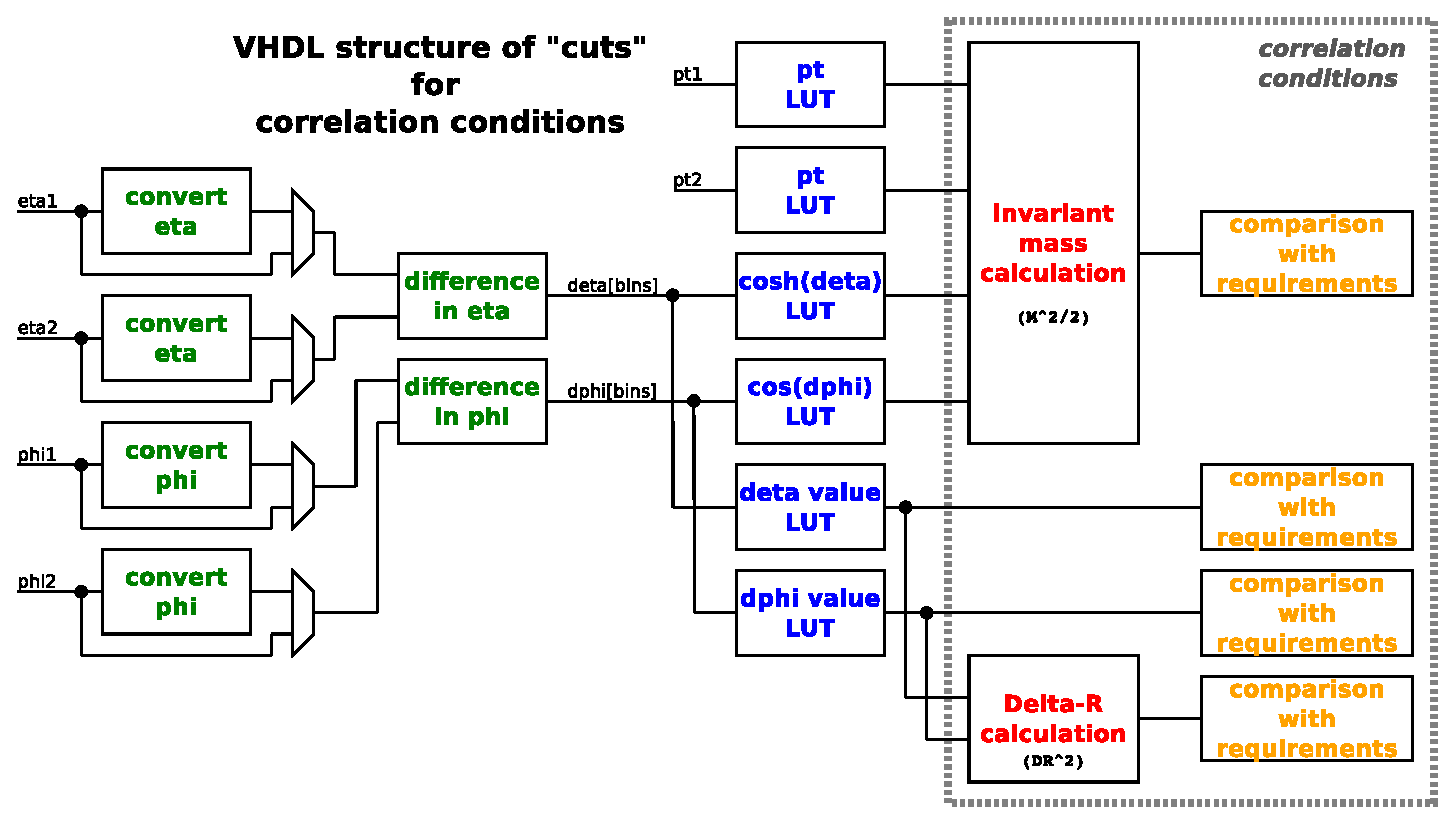
\includegraphics[width=15cm]{figures/scheme_vhdl_cuts_correllation_condition}
\caption{VHDL structure of cuts for correlation conditions}
\label{fig:gtl:scheme_vhdl_cuts_correllation_condition}
\end{figure}

\textbf{Overview of correlation cuts in conditions}
\label{sec:gtl:overview_correlation_cuts}

The following list gives an overview of possible correlation cuts in conditions:

\begin{itemize}
\item Calo conditions:
\begin{itemize}
\item two-body pt (for double condition)
\end{itemize}
\item Calo conditions overlap removal:
\begin{itemize}
\item $\Delta\eta$ overlap removal
\item $\Delta\varphi$ overlap removal
\item $\Delta$R overlap removal
\item two-body pt (for double condition)
\end{itemize}
\item Muon conditions:
\begin{itemize}
\item charge correlation
\item two-body pt (for double condition)
\end{itemize}
\item Calo calo correlation condition with calo overlap removal:
\begin{itemize}
\item $\Delta\eta$ overlap removal
\item $\Delta\varphi$ overlap removal
\item $\Delta$R overlap removal
\item $\Delta\eta$
\item $\Delta\varphi$
\item $\Delta$R
\item invariant mass
\item two-body pt
\end{itemize}
\item Calo calo correlation condition:
\begin{itemize}
\item $\Delta\eta$
\item $\Delta\varphi$
\item $\Delta$R
\item invariant mass
\item two-body pt
\end{itemize}
\item Calo calo correlation condition for invariant mass divided by $\Delta$R:
\begin{itemize}
\item invariant mass divided by $\Delta$R
\end{itemize}
\item Calo calo correlation condition mass with three objects:
\begin{itemize}
\item invariant mass with three objects
\end{itemize}
\item Calo muon correlation condition:
\begin{itemize}
\item $\Delta\eta$
\item $\Delta\varphi$
\item $\Delta$R
\item invariant mass
\item two-body pt
\end{itemize}
\item Calo esums correlation condition:
\begin{itemize}
\item $\Delta\varphi$
\item transverse mass
\item two-body pt
\end{itemize}
\item Muon muon correlation condition:
\begin{itemize}
\item charge correlation
\item $\Delta\eta$
\item $\Delta\varphi$
\item $\Delta$R
\item invariant mass or invariant mass unconstraint pt
\item two-body pt
\end{itemize}
\item Muon muon correlation condition for invariant mass divided by $\Delta$R:
\begin{itemize}
\item charge correlation
\item invariant mass divided by $\Delta$R
\end{itemize}
\item Muon muon correlation condition mass with three objects:
\begin{itemize}
\item charge correlation
\item invariant mass with three objects
\end{itemize}
\item Muon esums correlation condition:
\begin{itemize}
\item $\Delta\varphi$
\item transverse mass
\item two-body pt
\end{itemize}
\end{itemize}

\paragraph{Correlation condition module}
\label{sec:gtl:correlation_condition_modules}

As described in section Correlation conditions (\ref{sec:gtl:correlation_conditions}), correlations of two object types are available. Therefore several correlations (objects 1-objects 2) are possible:
\begin{itemize}
\item Correlation condition with calorimeter objects\\
\egamma-\egamma, \egamma-jet, \egamma-tau, jet-jet, jet-tau and tau-tau.
\item Correlation condition with calorimeter objects and \esums (\etm, ET$_{miss}^{HF}$ and \htm only)\\
\egamma-etm, jet-etm, tau-etm, \egamma-htm, jet-htm, tau-htm, \egamma-etmhf, jet-etmhf and tau-etmhf.
\item Correlation condition with calorimeter objects and muons objects\\
\egamma-muon, jet-muon and tau-muon.
\item Correlation condition with muon objects\\
\item Correlation condition with muon objects and \esums (\etm, ET$_{miss}^{HF}$ and \htm only)\\
muon-etm, muon-etmhf and muon-htm.
\end{itemize}

There are two correlations for mass with three objects:
\begin{itemize}
\item Correlation condition for mass with three objects with calorimeter objects (same type, same bunch-crossing)\\
\item Correlation condition for mass with three objects with muon objects\\
\end{itemize}

In correlation condition with calorimeter and muons objects we have different scales of calorimeter and muon objects in $\eta$ and $\varphi$, therefore LUTs for conversion of the calorimeter bins to muon bins are used (in \href{\gitbranch/firmware/hdl/packages/gtl_pkg.vhd}{\texttt{\textquotesingle gtl\_pkg.vhd\textquotesingle }}:
 e.g. \small{EG\_ETA\_CONV\_2\_MUON\_ETA\_LUT}\normalsize  and \small{EG\_PHI\_CONV\_2\_MUON\_PHI\_LUT}\normalsize).\\\\
\textbf{Remark:}\\
The center value of bins are used as reference value for conversion.
The content of \small{EG\_ETA\_CONV\_2\_MUON\_ETA\_LUT}\normalsize is calculated with formular:\\ "converted-calo-eta[bin] = calo-eta[bin] $\times$ 4 + 2",\\
of \small{EG\_PHI\_CONV\_2\_MUON\_PHI\_LUT}\normalsize with formular:\\
"converted-calo-phi[bin] = calo-phi[bin] $\times$ 4 + 2".\\
Definitions of scales (see Tables \ref{tab:gtl:calo_eta_scale_new}, \ref{tab:gtl:calo_phi_scale}, \ref{tab:gtl:muon_eta_scale} and \ref{tab:gtl:muon_phi_scale}):
\begin{itemize}
\item Calorimeter objects:
    \begin{itemize}
    \item $\eta$ bin width = $\frac{0.087}{2}$ (bin 0 from 0.0 to $\frac{0.087}{2}$)
    \item $\phi$ bin width = $\frac{2\pi}{144}$ (bin 0 from 0.0 to $\frac{2\pi}{144}$)
    \end{itemize}
\item Muon objects:
    \begin{itemize}
    \item $\eta$ bin width = $\frac{0.087}{8}$ (bin 0 from \small{0.5}$\times\frac{-0.087}{8}$ to \small{0.5}$\times\frac{+0.087}{8}$)
    \item $\phi$ bin width = $\frac{2\pi}{576}$ (bin 0 from 0.0 to $\frac{2\pi}{576}$)
    \end{itemize}
\end{itemize}

\begin{figure}[htb]
\centering
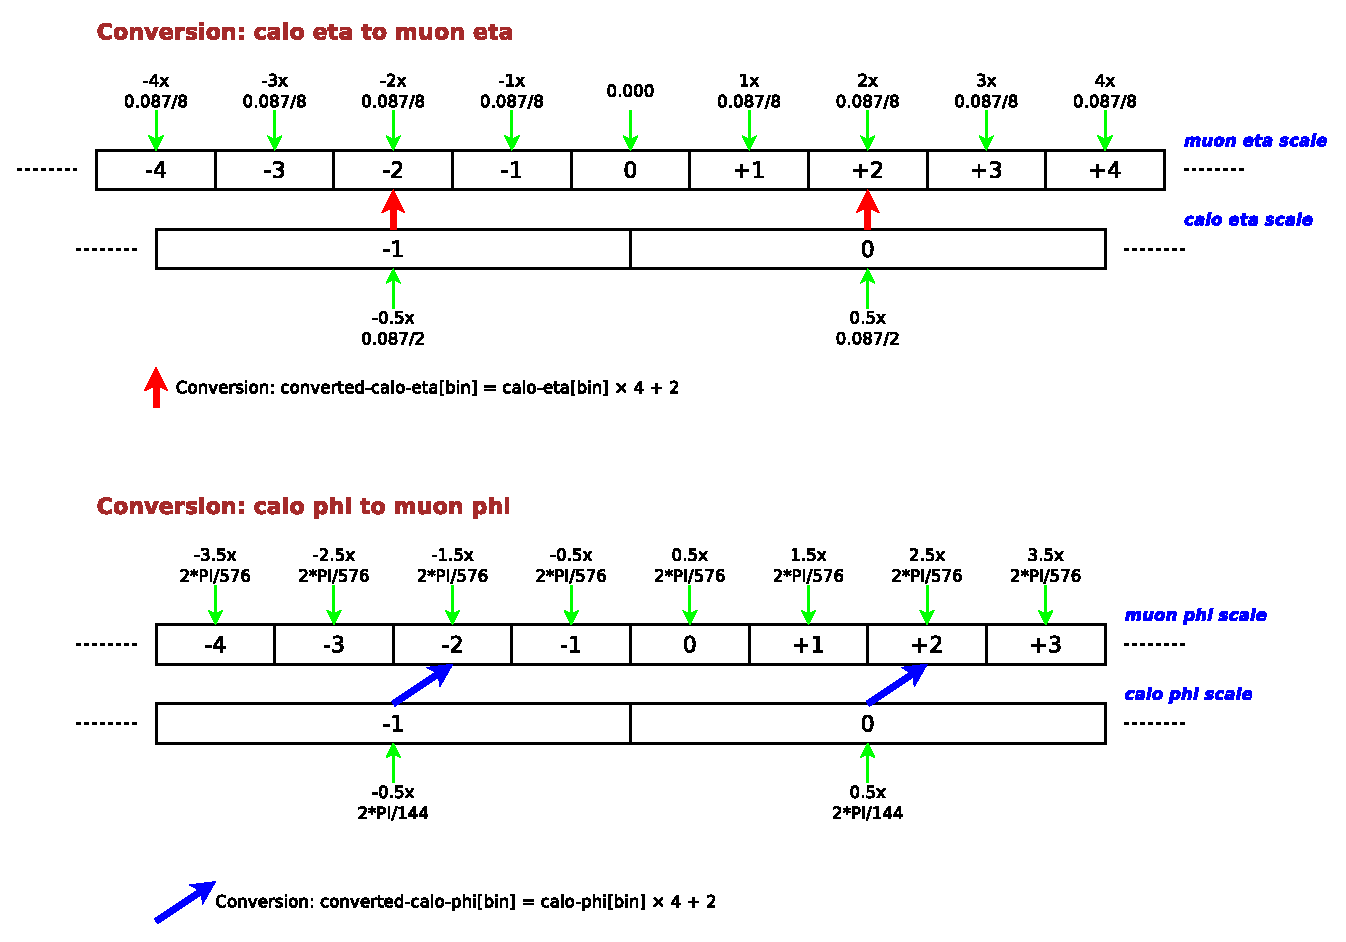
\includegraphics[width=15cm]{figures/convert_scheme_calo_2_muon_eta_phi}
\caption{Conversion of calorimeter $\eta$ and $\varphi$ to muon scales}
\label{fig:gtl:convert_scheme_calo_2_muon_eta_phi}
\end{figure}

\clearpage

\subsubsection{External Conditions}
\label{sec:gtl:external_conditions}
Maximal 256 External Conditions are possible in \gt. They are provided as inputs in the Algorithms logic of \ugtl.
External Conditions will include the "Technical Trigger" of the legacy system.

\subsubsection{Algorithms logic}
\label{sec:gtl:algorithms_logic}

The outputs of all the instantiated conditions are combined in the Algorithms logic with boolean algebra given by TME for every single Algorithm. These Algorithms are registered and provided as inputs for \fdl.

\clearpage
